%% V0.1
%% 2020/10/09
%% by Markus Götz, Björn Hagemeier, James Kahn

\documentclass[aspectratio=1610]{beamer}
\usepackage{helmholtzai}

\title{High-performance Data Analysis with GPUs}
\subtitle{KSETA Topical Courses March 2021}
\author{Markus Götz}
\date{2021-03-11}
\institute{Karlsruhe Institute of Technology (KIT)}

\usepackage{adjustbox}
\usepackage{tikz}

\usetikzlibrary{
    arrows, 
    positioning
}

\begin{document}

\maketitle

\begin{frame}
    \frametitle{Graphical Processing Unit (GPU)}
    \framesubtitle{A Brief History Primer}
    
    \begin{columns}
        \begin{column}{0.48\textwidth}
            \begin{figure}
                \centering
                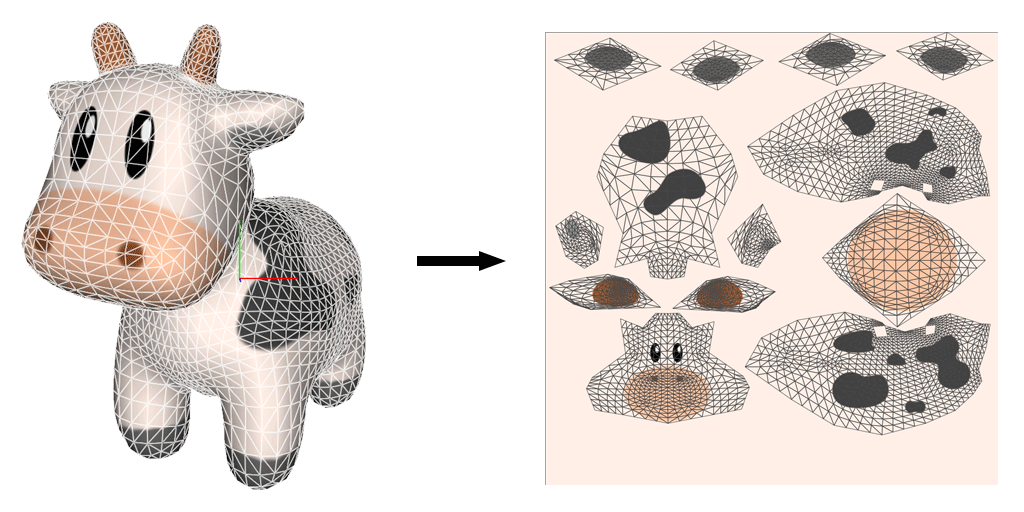
\includegraphics[width=0.8\linewidth]{images/cg.png}
                
                \source{Warren Moore, "Textures and Samples in Metal", 2014.}
            \end{figure}
            \begin{figure}
                \centering
                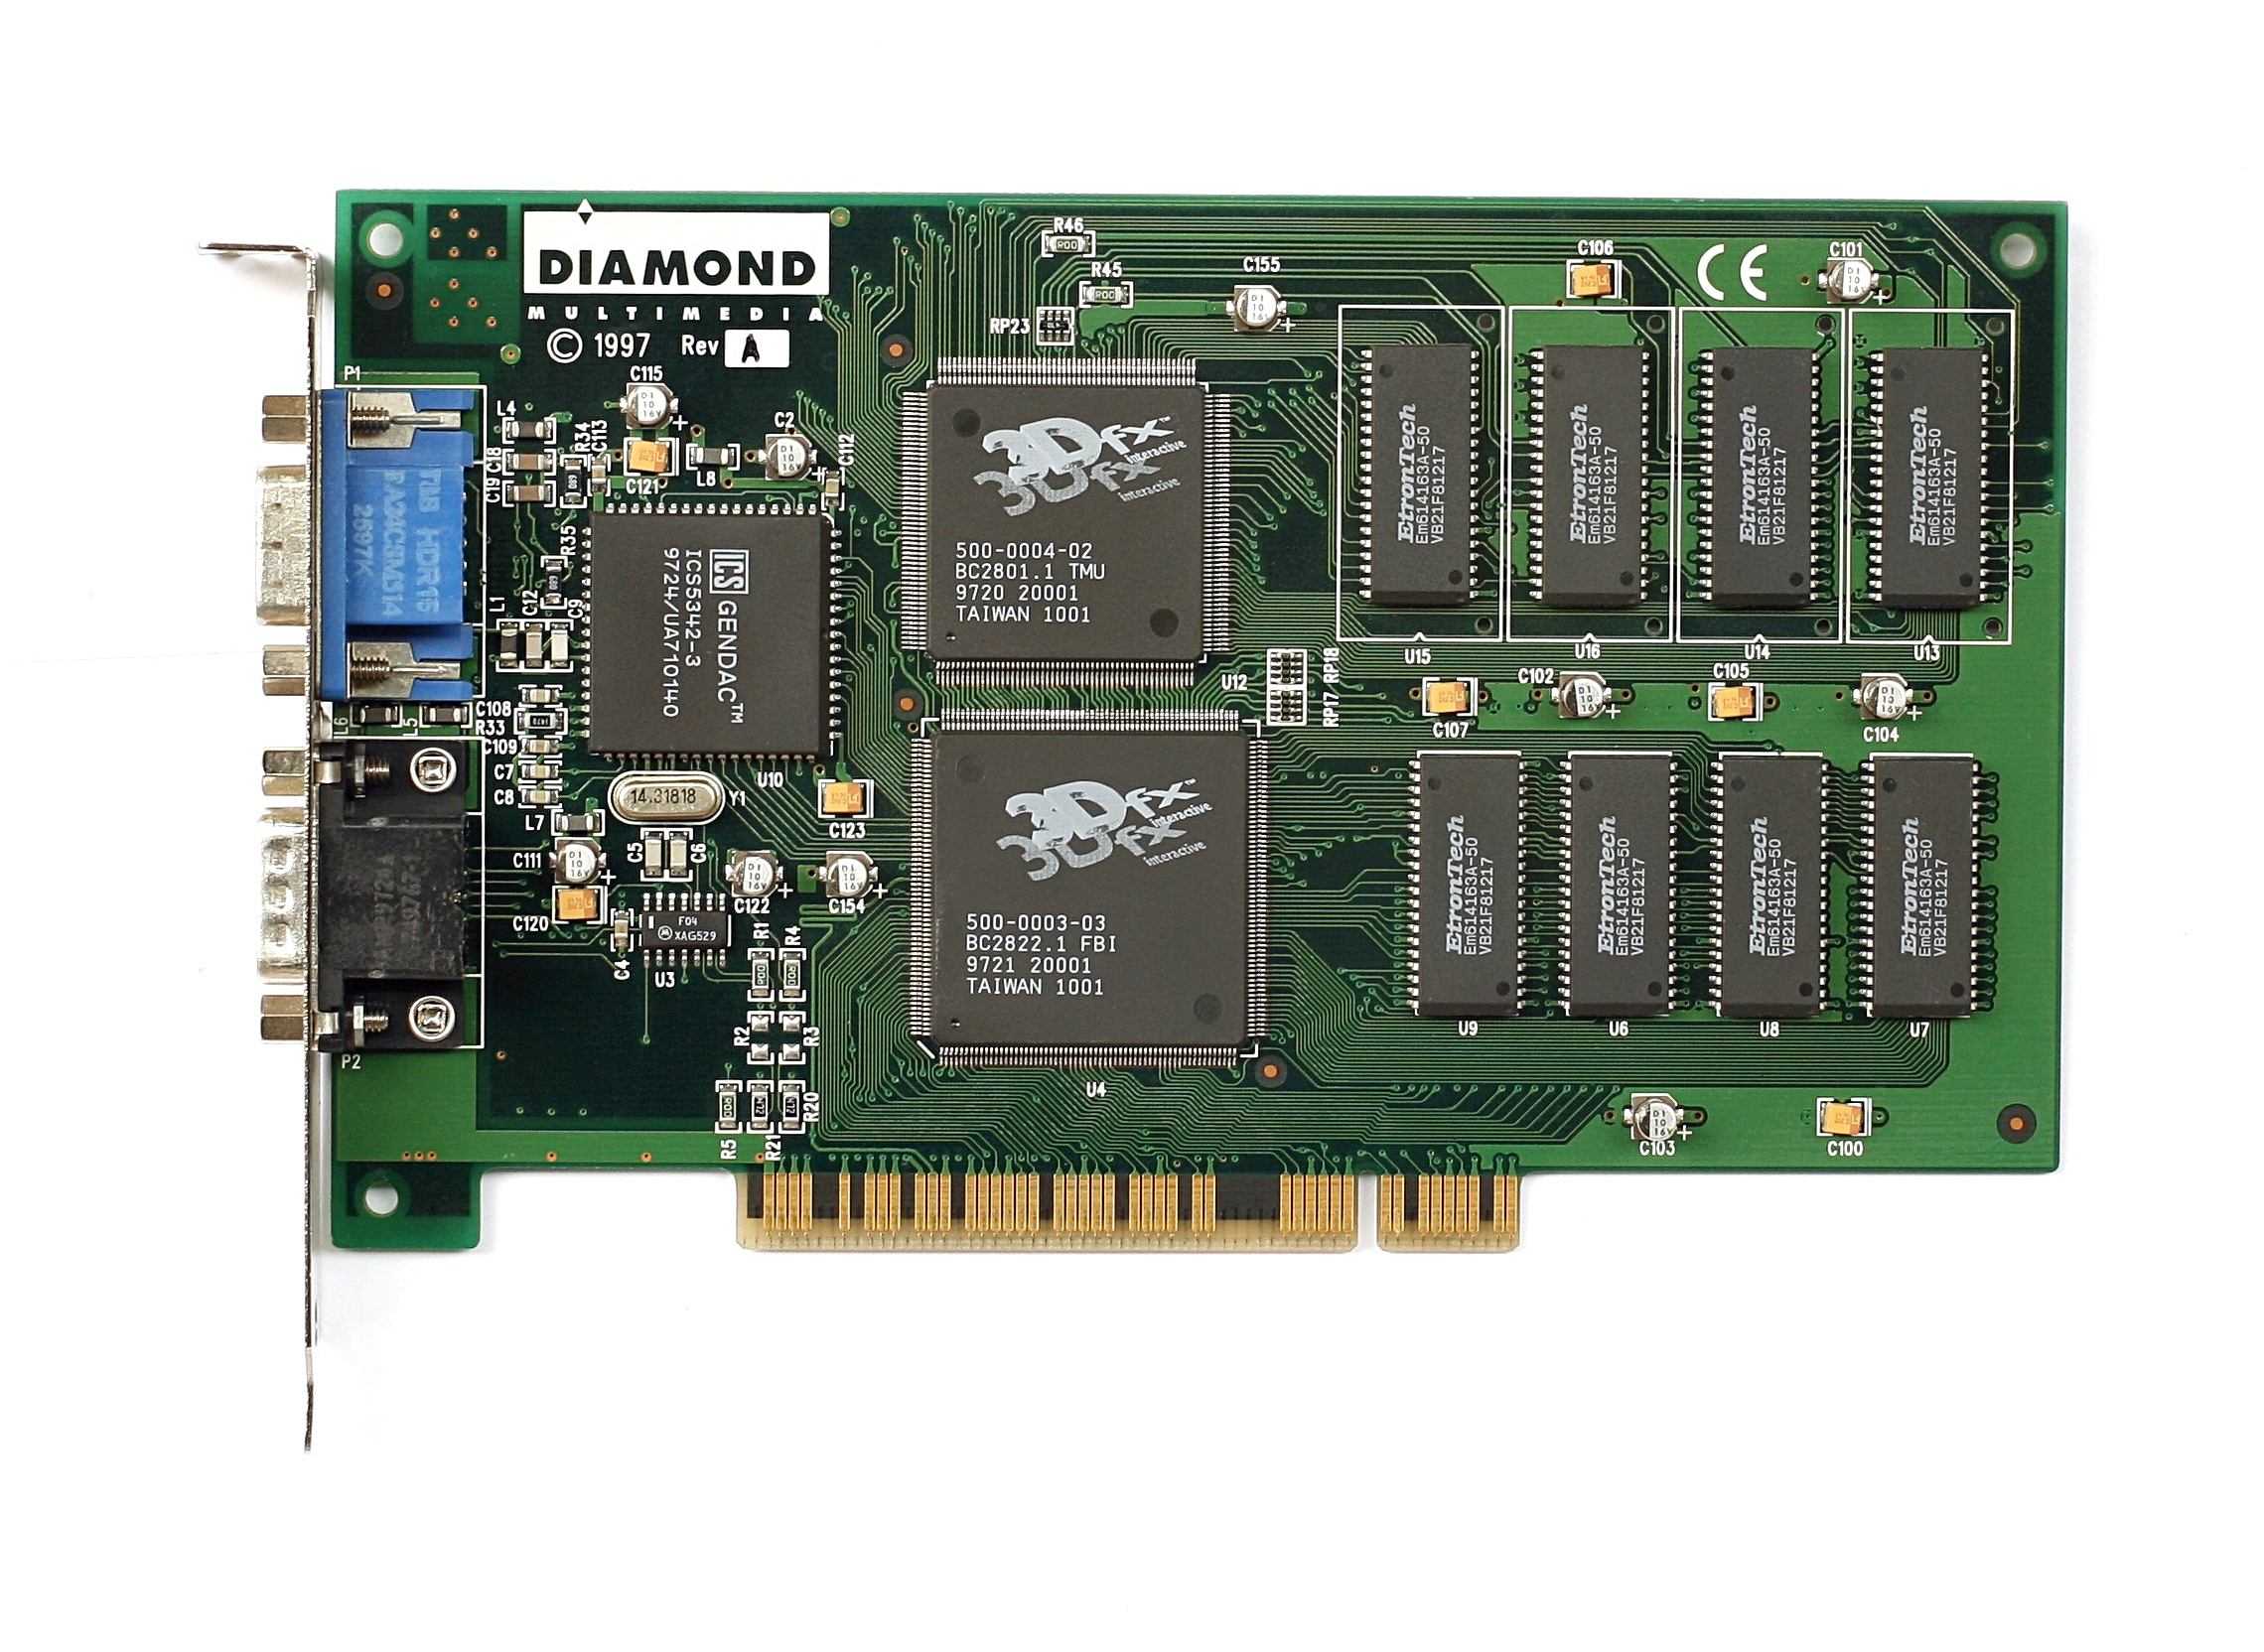
\includegraphics[width=0.6\textwidth]{images/voodoo.jpg}
                
                \source{Konstantin Lanzet, Wikipedia, "3dfx Voodoo Graphics"}
            \end{figure}
        \end{column}
        \begin{column}{0.48\textwidth}
            \begin{itemize}
                \item Early 1990s \textbf{real-time rendering}
                \begin{itemize}
                    \item Highly computational intensive
                    \item CPU did all the work\\~
                \end{itemize}
                \item Introduction of \textbf{dedicated hardware}
                \begin{itemize}
                    \item NVidia coined the term \textbf{GPU}
                    \item Short and repeated algorithms
                    \item Massively parallel vector operations\\~
                \end{itemize}
                \item Repurpose for ``regular'' problems
                \begin{itemize}
                    \item Express problem as an image
                    \item Flexible programming advancements, e.g. non-fixed function pipelines\\~
                \end{itemize}
            \end{itemize}
        \end{column}
    \end{columns}
\end{frame}

\begin{frame}
    \frametitle{Graphical Processing Unit (GPU)}
    \framesubtitle{CPUs versus GPUs}
    
    \begin{figure}
        \centering
        \begin{tikzpicture}
            \node[fill=hgfblue20, draw=hgfblue, minimum width=2.4cm, minimum height=1.0cm] at (1.2, 1.7) {\footnotesize Core 1};
            \node[fill=hgfblue20, draw=hgfblue, minimum width=2.4cm, minimum height=1.0cm] at (3.8, 1.7) {\footnotesize Core 2};
            \node[fill=hgfblue20, draw=hgfblue, minimum width=2.4cm, minimum height=1.0cm] at (1.2, 0.5) {\footnotesize Core 3};
            \node[fill=hgfblue20, draw=hgfblue, minimum width=2.4cm, minimum height=1.0cm] at (3.8, 0.5) {\footnotesize Core 4};
            \node[fill=hgfblue60, draw=hgfblue, minimum width=5cm, minimum height=0.5cm] at (2.5, -0.5) {\footnotesize DRAM};
            \node at (2.5, -1.2) {CPU};
            \node[draw=hgfblue, minimum width=5.4cm, minimum height=4.0cm] at (2.5, 0.4) {};
            \node at (2.5, -2.9) {~};
        \end{tikzpicture}
        \qquad
        \begin{tikzpicture}
            \fill [fill=hgfblue20] (0,0) -- (5.0,0) -- (5.0,5.0) -- (0,5.0) -- cycle;
            \draw[step=0.1cm, color=hgfblue] (0,0) grid (5.0,5.0);
            \node[fill=hgfblue60, draw=hgfblue, minimum width=5cm, minimum height=0.5cm] at (2.5, -0.5) {\footnotesize VRAM};
            \node at (2.5, -1.2) {GPU};
            \node[draw=hgfblue, minimum width=5.4cm, minimum height=6.8cm] at (2.5, 1.8) {};
        \end{tikzpicture}
    \end{figure}
\end{frame}

\begin{frame}
    \frametitle{Graphical Processing Unit (GPU)}
    \framesubtitle{CPUs versus GPUs}
    
    \begin{columns}
        \begin{column}{0.48\textwidth}
            \begin{figure}
                \centering
                \begin{tikzpicture}
                    \fill [fill=hgfblue20] (0,0) -- (5.0,0) -- (5.0,5.0) -- (0,5.0) -- cycle;
                    \draw[step=0.1cm, color=hgfblue] (0,0) grid (5.0,5.0);
                    \node[fill=hgfblue60, draw=hgfblue, minimum width=5cm, minimum height=0.5cm] at (2.5, -0.5) {\footnotesize VRAM};
                    \node at (2.5, -1.2) {GPU};
                    \node[draw=hgfblue, minimum width=5.4cm, minimum height=6.8cm] at (2.5, 1.8) {};
                \end{tikzpicture}
            \end{figure}
        \end{column}
        \begin{column}{0.48\textwidth}
            \begin{itemize}
                \item<+-> \textbf{CPU}---Central Processing Unit
                \begin{itemize}
                    \item<.-> Low number of strong cores
                    \item<.-> Independent and vector computation
                    \item<.-> Low to medium parallelization\\~
                \end{itemize}
                \item<.-> \textbf{GPU}---Graphical Processing Unit
                \begin{itemize}
                    \item<.-> High number of weak cores
                    \item<.-> Designed for vector operations
                    \item<.-> Lock-step mode
                    \item<.-> High parallelization\\~
                \end{itemize}
            
                \item<+-> $\rightarrow$ \emph{race car} vs \emph{transport train}
            \end{itemize}
        \end{column}
    \end{columns}
\end{frame}

\begin{frame}
    \frametitle{Graphical Processing Unit (GPU)}
    \framesubtitle{Theoretical Peak Performance, Double Precision}
    
    \begin{figure}
        \centering
        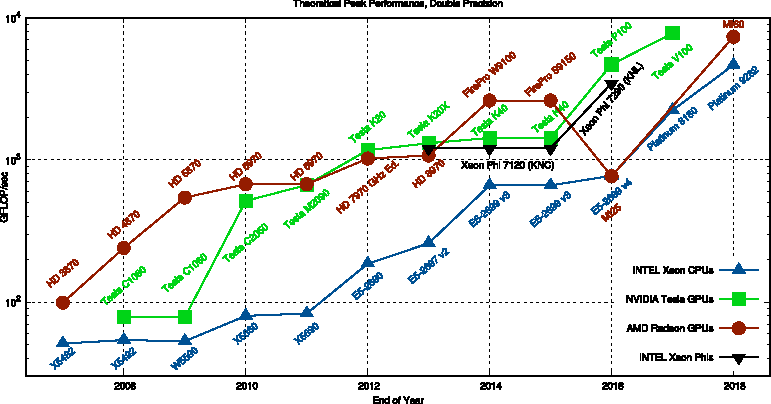
\includegraphics[height=0.95\textheight]{images/gpu-peak-performance.pdf}
        
        \source{Karl Rupp, CPU/GPU Performance Comparison, https://www.karlrupp.net/2013/06/cpu-gpu-and-mic-hardware-characteristics-over-time/.}
    \end{figure}
\end{frame}

\begin{frame}
    \frametitle{Graphical Processing Unit (GPU)}
    \framesubtitle{Theoretical Memory Bandwidth}
    
    \begin{figure}
        \centering
        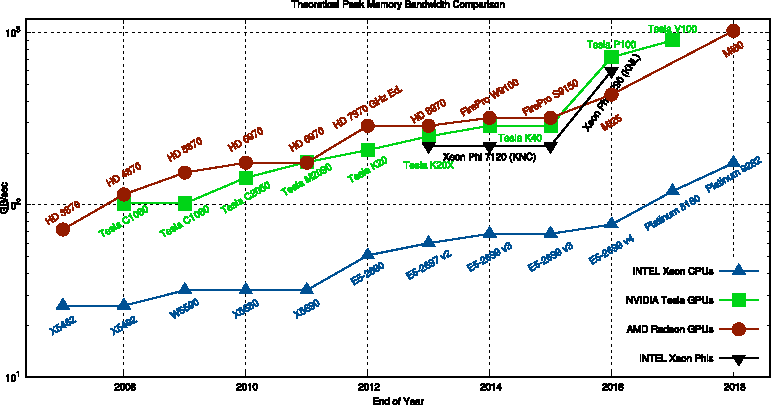
\includegraphics[height=0.95\textheight]{images/gpu-memory-bandwidth.pdf}
        
        \source{Karl Rupp, CPU/GPU Performance Comparison, https://www.karlrupp.net/2013/06/cpu-gpu-and-mic-hardware-characteristics-over-time/.}
    \end{figure}
\end{frame}

\begin{frame}
    \frametitle{Programming GPUs}
    \framesubtitle{Processing Flow}
    
    \begin{columns}
        \begin{column}{0.28\textwidth}
            \begin{figure}
                \centering
                \begin{tikzpicture}
                    \node[fill=hgfblue20, draw=hgfblue, minimum width=1.2cm, minimum height=0.5cm] at (0.6, 4.8) {\tiny Core 1};
                    \node[fill=hgfblue20, draw=hgfblue, minimum width=1.2cm, minimum height=0.5cm] at (1.9, 4.8) {\tiny Core 2};
                    \node[fill=hgfblue20, draw=hgfblue, minimum width=1.2cm, minimum height=0.5cm] at (0.6, 4.2) {\tiny Core 3};
                    \node[fill=hgfblue20, draw=hgfblue, minimum width=1.2cm, minimum height=0.5cm] at (1.9, 4.2) {\tiny Core 4};
                    \node[fill=hgfblue60, draw=hgfblue, minimum width=2.5cm, minimum height=0.25cm] at (1.25, 3.6) {\tiny DRAM};
                    \node at (1.25, 3.2) {\tiny CPU};
                    \node[draw=hgfblue, minimum width=2.7cm, minimum height=2.2cm] (cpu) at (1.25, 4.1) {};
                    
                    \foreach \x in {0, ..., 16}
                    {
                        \fill [fill=hgfblue20] (0,\x*0.15) -- (2.5,\x*0.15) -- (2.5,\x*0.15+0.1) -- (0,\x*0.15+0.1) -- cycle;
                        \draw[step=0.05cm, color=hgfblue] (0,\x*0.15) grid (2.5,\x*0.15+0.1);
                    }
                    
                    \node[fill=hgfblue60, draw=hgfblue, minimum width=2.5cm, minimum height=0.25cm] at (1.25, -0.25) {\tiny VRAM};
                    \node at (1.25, -0.6) {\tiny GPU};
                    \node[draw=hgfblue, minimum width=2.7cm, minimum height=3.4cm] (gpu) at (1.25, 0.9) {};
                    
                    \draw[>=stealth, <->, color=hgfblue] (gpu.north) -- (cpu.south);
                \end{tikzpicture}
            \end{figure}
        \end{column}
        \begin{column}{0.48\textwidth}
            \begin{itemize}
                \item GPU is accelerator card
                \begin{itemize}
                    \item \textbf{Separate entity}, connected via bus
                    \item Computations controlled by CPU\\~
                \end{itemize}
                \item \textbf{Template processing workflow}
                \begin{enumerate}
                    \item Transfer data from CPU to GPU
                    \item Load GPU program and execute
                    \item Transfer results from GPU to CPU\\~
                \end{enumerate}
                \item CPU is independent
                \begin{itemize}
                    \item Concurrent other computations
                    \item Explicitly synchronization
                \end{itemize}
            \end{itemize}
        \end{column}
    \end{columns}
\end{frame}

\begin{frame}
    \frametitle{Programming GPUs}
    \framesubtitle{Caveats}
    
    \begin{columns}
        \begin{column}{0.28\textwidth}
            \begin{figure}
                \centering
                \begin{tikzpicture}
                    \node[fill=hgfblue20, draw=hgfblue, minimum width=1.2cm, minimum height=0.5cm] at (0.6, 4.8) {\tiny Core 1};
                    \node[fill=hgfblue20, draw=hgfblue, minimum width=1.2cm, minimum height=0.5cm] at (1.9, 4.8) {\tiny Core 2};
                    \node[fill=hgfblue20, draw=hgfblue, minimum width=1.2cm, minimum height=0.5cm] at (0.6, 4.2) {\tiny Core 3};
                    \node[fill=hgfblue20, draw=hgfblue, minimum width=1.2cm, minimum height=0.5cm] at (1.9, 4.2) {\tiny Core 4};
                    \node[fill=hgfblue60, draw=hgfblue, minimum width=2.5cm, minimum height=0.25cm] at (1.25, 3.6) {\tiny DRAM};
                    \node at (1.25, 3.2) {\tiny CPU};
                    \node[draw=hgfblue, minimum width=2.7cm, minimum height=2.2cm] (cpu) at (1.25, 4.1) {};
                    
                    \foreach \x in {0, ..., 16}
                    {
                        \fill [fill=hgfblue20] (0,\x*0.15) -- (2.5,\x*0.15) -- (2.5,\x*0.15+0.1) -- (0,\x*0.15+0.1) -- cycle;
                        \draw[step=0.05cm, color=hgfblue] (0,\x*0.15) grid (2.5,\x*0.15+0.1);
                    }
                    
                    \node[fill=hgfblue60, draw=hgfblue, minimum width=2.5cm, minimum height=0.25cm] at (1.25, -0.25) {\tiny VRAM};
                    \node at (1.25, -0.6) {\tiny GPU};
                    \node[draw=hgfblue, minimum width=2.7cm, minimum height=3.4cm] (gpu) at (1.25, 0.9) {};
                    
                    \draw[>=stealth, <->, color=hgfblue] (gpu.north) -- (cpu.south);
                \end{tikzpicture}
            \end{figure}
        \end{column}
        \begin{column}{0.48\textwidth}
            \begin{itemize}
                \item \textbf{Lock-step} computation
                \begin{itemize}
                    \item Processors are technically grouped
                    \item Diverging processing, e.g. \texttt{if-else}-clause, causes waiting\\~
                \end{itemize}
                \item \textbf{Memory hierarchy}
                \begin{itemize}
                    \item Actually three memory levels
                    \item Unified address space at performance cost\\~
                \end{itemize}
                \item \textbf{Limits to parallelization}
                \begin{itemize}
                    \item Unsuitable computation problem
                    \item Computation-communication-hiding
                \end{itemize}
            \end{itemize}
        \end{column}
    \end{columns}
\end{frame}

\begin{frame}
    \frametitle{Programming GPUs}
    \framesubtitle{Programming Models and APIs}
    
    \begin{columns}
        \begin{column}{0.48\textwidth}
            \begin{figure}
                \centering
                \begin{tikzpicture}
                    \node[draw=hgfblue, fill=hgfblue40, minimum width=5cm] (hll) at (0.0, 4.5) {High-level libraries};
                    \node[draw=hgfblue, fill=hgfblue40, minimum width=5cm] (hlp) at (0.0, 3.0) {High-level platform};
                    \node[draw=hgfblue, fill=hgfblue40, minimum width=5cm] (lll) at (0.0, 1.5) {Low-level libraries};
                    \node[draw=hgfblue, fill=hgfblue40, minimum width=5cm] (llp) at (0.0, 0.0) {Low-level platform};
                    \node[draw=hgfblue, minimum width=6cm, minimum height=6.5cm] at (0.0, 2.0) {};
                    \node at (0.0, -0.85) {\textbf{GPU Programming}};
                    
                    \draw[>=stealth, ->, draw=hgfblue] (llp.north) -- (lll.south);
                    \draw[>=stealth, ->, draw=hgfblue] (lll.north) -- (hlp.south);
                    \draw[>=stealth, ->, draw=hgfblue] (hlp.north) -- (hll.south);
                \end{tikzpicture}
            \end{figure}
        \end{column}
        \begin{column}{0.48\textwidth}
            \begin{itemize}
                \item Scripting languages, algorithms
                \item Examples: RAPIDS, HeAT, \\~
            
                \item Bindings for device primitives
                \item Examples: CuPy, Numba, JuliaGPU\\~
                
                \item Low-level language, algorithms
                \item Examples: Thrust, CuBLAS, Gingko\\~
                
                \item Direct API to device primitives
                \item Examples: CUDA, HIP, OpenCL
            \end{itemize}
        \end{column}
    \end{columns}
\end{frame}

\begin{frame}
    \frametitle{Programming GPUs -- Low-level Platform}
    \framesubtitle{Compute Unified Device Architecture (CUDA)}
    
    \begin{columns}
        \begin{column}{0.48\textwidth}
            \begin{figure}
                \centering
                
\includegraphics[width=0.7\linewidth]{images/cuda.png}
                
                \source{https://nvidia.com}
            \end{figure}
        \end{column}
        \begin{column}{0.48\textwidth}
            \begin{itemize}
                \item \textbf{Proprietary NVidia API}
                \begin{itemize}
                    \item General purpose GPU programming
                    \item Introduced first in 2007
                    \item Current version: 11.0\\~
                \end{itemize}
                \item Available for C/C++
                \begin{itemize}
                    \item Modification of base languages
                    \item Requires custom \texttt{nvcc} compiler\\~
                \end{itemize}
                \item Most widely used API, $\approx$\textbf{25\% share} on Top-500 \textbf{supercomputers} (2019)
            \end{itemize}
        \end{column}
    \end{columns}
\end{frame}

\begin{frame}[fragile]
    \frametitle{Low-level Platforms}
    \framesubtitle{CUDA Example}
    
    \begin{lstlisting}[language=C++, basicstyle=\ttfamily\upshape\tiny]
__global__ void add(int n, float *x, float *y) {
    int index = threadIdx.x;
    int stride = blockDim.x;
    for (int i = index; i < n; i += stride)
        y[i] = x[i] + y[i];
}

int main(void) {
    int N = 1<<20;
    float *x, *y;
    
    // Allocate Unified Memory – accessible from CPU or GPU
    cudaMallocManaged(&x, N*sizeof(float)); 
    cudaMallocManaged(&y, N*sizeof(float));
    // initialize x and y arrays on the host
    for (int i = 0; i < N; i++) {
        x[i] = 1.0f;
        y[i] = 2.0f;
    }
    // Run kernel on 1M elements on the GPU
    add<<<1, 256>>>(N, x, y);
    
    // Wait for GPU to finish before accessing on host
    cudaDeviceSynchronize();
    // Free memory
    cudaFree(x); 
    cudaFree(y);
    
    return 0;
}
    \end{lstlisting}
    \vspace{-0.5em}
    \source{NVidia©, modified example from: https://developer.nvidia.com/blog/even-easier-introduction-cuda/}
\end{frame}

\begin{frame}
    \frametitle{High-level Platforms}
    \framesubtitle{Tensor Computation Frameworks}
    
    \begin{columns}
        \begin{column}{0.58\textwidth}
            \begin{itemize}
                \item Access GPU from scripting languages
                \begin{itemize}
                    \item Predominantly in Python
                    \item Wrappers around low-level calls\\~
                \end{itemize}
                \item Abstraction: \textbf{multi-dimensional tensors}\\~
                \item Application areas
                \begin{itemize}
                    \item \textbf{Deep learning}
                    \item Simulations
                    \item $\cdots$\\~
                \end{itemize}
                \item Different computational backends
                \begin{itemize}
                    \item All: CPU and GPU
                    \item Additionally: TPU, FPGA, IPU
                \end{itemize}
            \end{itemize}
        \end{column}
        \begin{column}{0.38\textwidth}
            \begin{figure}
                \centering
                
\includegraphics[width=0.8\linewidth]{images/pytorch.png}
                
                \source{https://pytorch.org}
            \end{figure}
            \begin{figure}
                \centering
                
\includegraphics[width=0.8\linewidth]{images/tensorflow.png}
                
                \source{https://tensorflow.org}
            \end{figure}
            \begin{figure}
                \centering
                
\includegraphics[width=0.7\linewidth]{images/mxnet.png}
                
                \source{https://mxnet.apache.org}
            \end{figure}
        \end{column}
    \end{columns}
\end{frame}

\begin{frame}
    \frametitle{PyTorch}
    \framesubtitle{Overview}
    
    \begin{columns}
        \begin{column}{0.48\textwidth}
            \begin{itemize}
                \item Why PyTorch?
                \begin{itemize}
                    \item Currently \textbf{fastest} implementation
                    \item Largest \textbf{community} in users
                    \item Wide adoption in research\\~
                \end{itemize}
                \item Specifics computational features
                \begin{itemize}
                    \item \textbf{Eager computation}
                    \item Tight integration with NumPy
                    \item Strong sparse tensor support\\~
                \end{itemize}
                \item Tooling and libraries around PyTorch
                \begin{itemize}
                    \item Debuggers and performance profiling
                    \item Bayesian approaches, e.g. \texttt{pyro}
                \end{itemize}
            \end{itemize}
        \end{column}
        \begin{column}{0.48\textwidth}
            \begin{figure}
                \centering
                \begin{figure}
                    \centering
                    
\includegraphics[width=0.95\linewidth]{images/pytorch.png}
                \end{figure}
            \end{figure}
        \end{column}
    \end{columns}
\end{frame}

\begin{frame}[fragile]
    \frametitle{PyTorch}
    \framesubtitle{Tensor Initialization}
    
    \begin{onlyenv}<1->
    \begin{lstlisting}[language=Python]
>>> import torch
>>> vector = torch.arange(10)
>>> vector 
tensor([0, 1, 2, 3, 4, 5, 6, 7, 8, 9])
    \end{lstlisting}
    \end{onlyenv}
    \vspace{1em}
    \begin{onlyenv}<2->
    \begin{lstlisting}[language=Python]
>>> import torch
>>> matrix = torch.tensor([
        [1, 2, 3, 4],
        [5, 6, 7, 8]
    ])
>>> matrix.shape
torch.Size([2, 4])
    \end{lstlisting}
    \end{onlyenv}
    \vspace{1em}
    \begin{onlyenv}<3->
        \begin{itemize}
            \item Various other initializers: \texttt{full(), one(), zeros(), rand(), ...}
        \end{itemize}
    \end{onlyenv}
\end{frame}

\begin{frame}[fragile]
    \frametitle{PyTorch}
    \framesubtitle{Meta Information}

    \begin{itemize}
        \item Information about the PyTorch tensor object itself
    \end{itemize}
    \vspace{1em}
    \begin{lstlisting}[language=Python]
>>> import torch
>>> volume = torch.randn((3, 4, 5,))
>>> volume.shape
torch.Size([3, 4, 5])

>>> volume.dtype
torch.float32

>>> volume.device
torch.device(type='cpu')
    \end{lstlisting}
\end{frame}

\section{Hands-on Part 1}

\begin{frame}[fragile]
    \frametitle{PyTorch}
    \framesubtitle{Element-wise Operations}
    
    \begin{itemize}
        \item PyTorch can operate on \textbf{multi-dimensional tensors} as \textbf{operands}\\~
        \item Avoids explicit looping, code resembles equations
    \end{itemize}
    \vspace{1em}
    \begin{lstlisting}[language=Python]
>>> import torch
>>> a = torch.arange(10)
>>> a
tensor([0, 1, 2, 3, 4, 5, 6, 7, 8, 9])

>>> b = torch.ones(10, dtype=a.dtype)
>>> b
tensor([1, 1, 1, 1, 1, 1, 1, 1, 1, 1])

>>> a + b
tensor([ 1, 2, 3, 4, 5, 6, 7, 8, 9, 10])
    \end{lstlisting}
\end{frame}

\begin{frame}[fragile]
    \frametitle{PyTorch}
    \framesubtitle{Broadcasting}
    
    \begin{itemize}
        \item PyTorch attempts to \textbf{broadcast} non-matching shapes\\~
        \item Dimensions equal to $1$ are repeated based on other operand
    \end{itemize}
    \vspace{1em}
    \begin{lstlisting}[language=Python]
>>> import torch
>>> vector = torch.arange(10)
>>> vector + 3
tensor([ 3,  4,  5,  6,  7,  8,  9, 10, 11, 12])
    \end{lstlisting}
\end{frame}

\begin{frame}[fragile]
    \frametitle{PyTorch}
    \framesubtitle{Slicing}
    
    \begin{itemize}
        \item \textbf{Slicing} a torch tensor allows to obtain partial tensor content
    \end{itemize}
    \vspace{1em}
    \begin{lstlisting}[language=Python]
>>> import torch
>>> matrix = torch.randn(size=(10, 3,))
>>> matrix[2]
tensor([1.2646, 0.4840, 0.4133])
    \end{lstlisting}
\end{frame}

\begin{frame}[fragile]
    \frametitle{PyTorch}
    \framesubtitle{Reduction Operations}
    
    \begin{itemize}
        \item \textbf{Reductions} combine all elements of tensors (or slices) to a singular output\\~
        \item Typical examples are: \texttt{max(), min(), sum(), ...}
    \end{itemize}
    \vspace{1em}
    \begin{lstlisting}[language=Python]
>>> import torch
>>> a = torch.arange(10)
>>> a
tensor([0, 1, 2, 3, 4, 5, 6, 7, 8, 9])

>>> a.sum()
tensor(45)
    \end{lstlisting}
\end{frame}

\section{Hands-on Part 2}

\begin{frame}[fragile]
    \frametitle{PyTorch}
    \framesubtitle{Using the GPU}

    \begin{itemize}
        \item PyTorch provides the \texttt{cuda} submodule to interact with CUDA
        \item Contains mostly the meta-information about the GPUs
    \end{itemize}
    \vspace{1em}
    \begin{lstlisting}[language=Python]
>>> import torch
>>> torch.cuda.is_available()
True

>>> torch.cuda.device_count()
1

>>> torch.cuda.get_device_name()
'A100-SXM4-40GB'
    \end{lstlisting}
\end{frame}

\begin{frame}[fragile]
    \frametitle{PyTorch}
    \framesubtitle{Moving Data between CPU and GPU}

    \begin{itemize}
        \item Data can be explicitly \textbf{moved} from \textbf{CPU} to \textbf{GPU} and vice versa\\~
        \item Some calls, e.g. \texttt{print()}, will do this automatically behind the scenes
    \end{itemize}
    \vspace{1em}
    \begin{lstlisting}[language=Python]
>>> import torch
>>> m = torch.arange(10)
>>> m.device
device(type='cpu')

>>> m_gpu = m.cuda()
>>> m_gpu.device
device(type='cuda:0')

>>> m_gpu.cpu().device
device(type='cpu')
    \end{lstlisting}
\end{frame}


\begin{frame}[fragile]
    \frametitle{PyTorch}
    \framesubtitle{Direct Data Allocation on GPU}
    
    \begin{itemize}
        \item Data can be directly allocated and/or moved to GPU\\~
        \item There are several approaches to do so
    \end{itemize}
    \vspace{1em}
    \begin{lstlisting}[language=Python]
>>> import torch
>>> torch.arange(2, device='cuda')
tensor([0, 1], device='cuda:0')

>>> torch.cuda.FloatTensor([1.0, 2.0])
tensor([1., 2.], device='cuda:0')

>>> torch.set_default_tensor_type('torch.cuda.FloatTensor')
>>> torch.randn(5).device
torch.device(type='cuda:0')
    \end{lstlisting}
\end{frame}

\begin{frame}[fragile]
    \frametitle{PyTorch}
    \framesubtitle{Computing on the GPU}
    
    \begin{itemize}
        \item PyTorch allows us to use the \textbf{same interface} for computation on GPU as on CPU
    \end{itemize}
    \vspace{1em}
    \begin{lstlisting}[language=Python]
>>> import torch
>>> a = torch.arange(10, device='cuda:0')
>>> a
tensor([0, 1, 2, 3, 4, 5, 6, 7, 8, 9], device='cuda:0')

>>> a.sum()
tensor(45, device='cuda:0')
    \end{lstlisting}
\end{frame}

\section{Hands-on Part 3}

\begin{frame}
    \frametitle{High-level Libraries}
    \framesubtitle{HeAT---A Distributed Tensor Framework}
    
    \begin{columns}
        \begin{column}{0.58\textwidth}
            \begin{itemize}
                \item \textbf{Python} framework for data-intesive computing
                \begin{itemize}
                    \item n-dimensional numerical tensors
                    \item Low-level operations and full-blown algorithms\\~
                \end{itemize}
                \item Joint development: \textbf{KIT-SCC, FZJ} and \textbf{DLR}\\~
                \item Transparent data-scaling via \textbf{MPI}
                \begin{itemize}
                    \item Start prototyping on laptop
                    \item Port without changes to HPC cluster
                    \item Data-parallelization strategy\\~
                \end{itemize}
                \item \textbf{Up to three orders of magnitude faster} than comparable frameworks (e.g. dask, \texttt{horovod})
            \end{itemize}
        \end{column}
        \begin{column}{0.38\textwidth}
            \begin{figure}
                \centering
                
\includegraphics[width=0.5\textwidth]{images/logo-heat.pdf}
            \end{figure}
            \begin{figure}
                \centering
                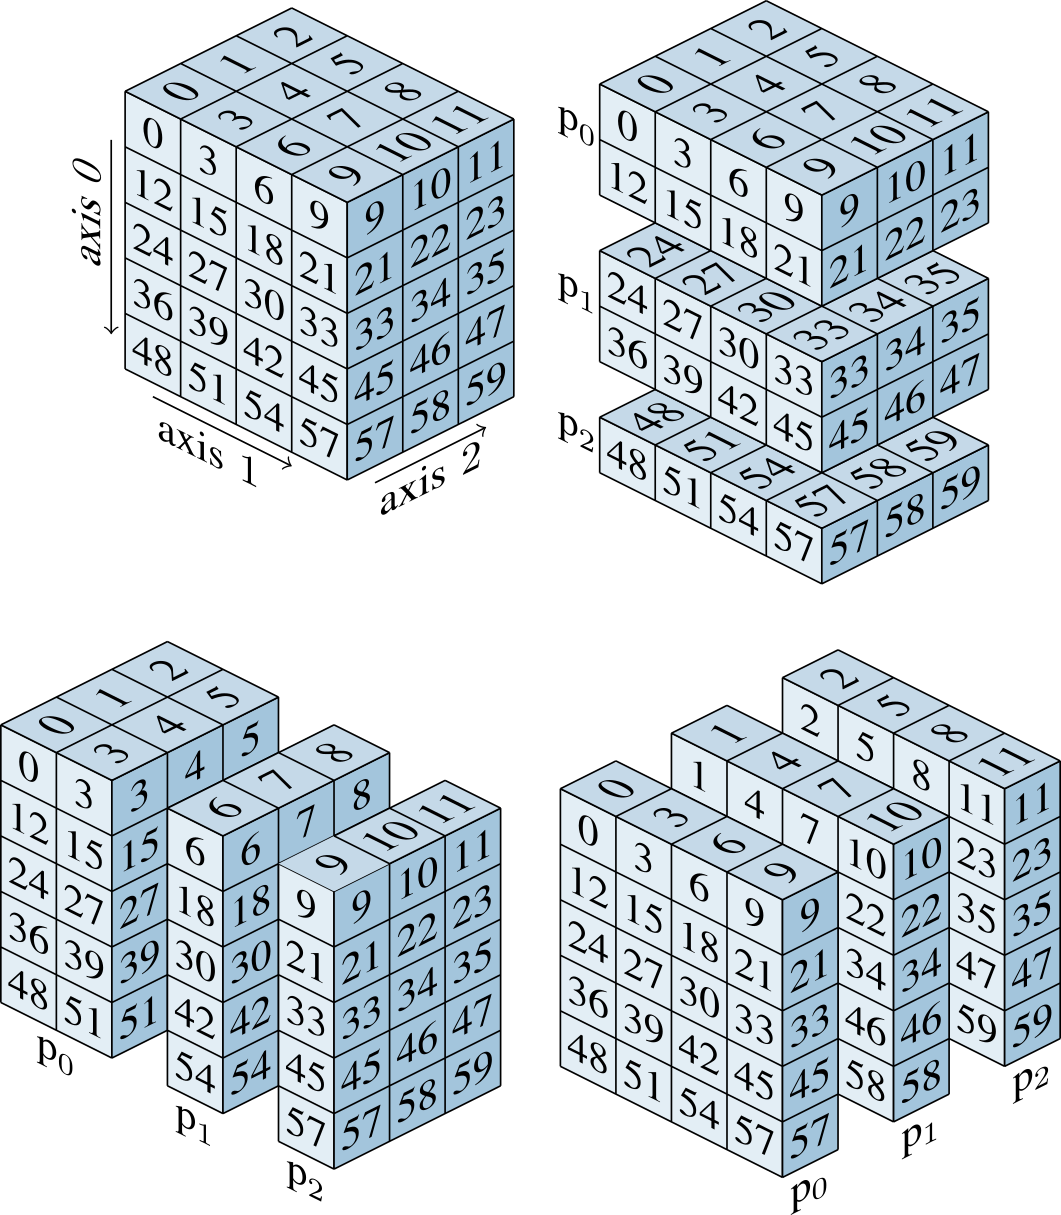
\includegraphics[width=0.8\textwidth]{images/all-splits.png}
            \end{figure}
        \end{column}
    \end{columns}
\end{frame}

\begin{frame}
    \frametitle{Conclusion}
    
    \begin{itemize}
        \item \textbf{GPUs} are massively \textbf{parallel} vector \textbf{co-processors}\\~
        \item Different approaches to programming
        \begin{itemize}
            \item High-level scripting, easy, less flexible and performant
            \item Low-level languages, difficult, maximal control and performance\\~
        \end{itemize}
        \item A large set of computational problems unsuitable for GPUs\\~
        \item \textbf{Benchmark, profile, debug!}
    \end{itemize}
\end{frame}

\begin{frame}[fragile]
    \frametitle{Get Your Own Hands Dirty...}
    \framesubtitle{...once again}
    
    \vspace{2em}
    Install the requirements first...
    \begin{lstlisting}[language=Bash]
pip install numpy torch
    \end{lstlisting}
    \vspace{1em}
    ... and clone the \textbf{slides} and \textbf{Jupyter notebooks}
    \begin{lstlisting}[language=Bash]
git clone https://github.com/Helmholtz-AI-Energy/kseta_2021.git
    \end{lstlisting}
    \vspace{1em}
    Available under the \emph{BSD-3 license}.
    
    \vspace{1em}
    \begin{figure}
        \centering
        
\includegraphics[height=0.25\textheight]{logos/scc.png}
    \end{figure}
\end{frame}

\end{document}
